\documentclass[../../Main.tex]{subfiles}

\begin{document}
    \begin{figure}[hbt!]
        \centerline{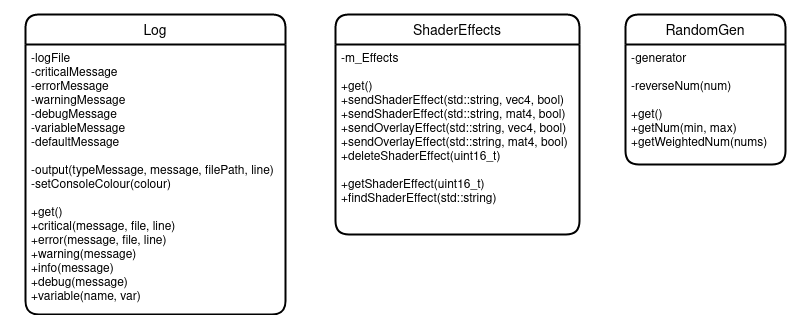
\includegraphics[scale=0.5]{img/Classes/Singletons.png}}
        \caption{Other singleton classes}
        \label{fig}
    \end{figure}
    Log
    \begin{center}
        Variables
        \begin{tabular}{ | m{0.45\textwidth} | m{0.45\textwidth} | }
            \hline
            \textbf{Variable Name} & \textbf{Description} \\
            \hline
            logFile & Stores the filename and location of the log file \\
            \hline
            criticalMessage & Stores the identifier for a critical message \\
            \hline
            errorMessage & Stores the identifier for an error message \\
            \hline
            warningMessage & Stores the identifier for a warning message \\
            \hline
            debugMessage & Stores the identifier for a debug message \\
            \hline
            variableMessage & Stores the identifier for a message with a variable \\
            \hline
            defaultMessage & Stores the default identifier \\
            \hline
        \end{tabular}
        Functions
        \begin{tabular}{ | m{0.15\textwidth} | m{0.35\textwidth}| m{0.4\textwidth} | }
            \hline
            \textbf{Function Name} & \textbf{Parameters} & \textbf{Description} \\
            \hline
            output & Takes in the identifier and the message as well as the filepath and the line of where the log occurred & Outputs the message in the correct format \\
            \hline
            setConsoleColour & A colour & Sets the console to the colour given (in debug mode for the terminal) \\
            \hline
            get & & Returns the only instance of the Log class \\
            \hline
            critical & Takes in the message and information for debugging & Uses the output function to output a critical message \\
            \hline
            error & Takes in the message and information for debugging & Uses the output function to output an error message \\
            \hline
            warning & Takes in the message & Uses the output function to output a warning \\
            \hline
            info & Takes in a message & Uses the output function to output a message \\
            \hline
            debug & Takes in a message & Uses the output function to output a debug message \\
            \hline
            variable & Takes in the name of the variable and the variable & Uses the output function to output a variable \\
            \hline
        \end{tabular}
    \end{center}
    ShaderEffectsManager
    \begin{center}
        Variables
        \begin{tabular}{ | m{0.45\textwidth} | m{0.45\textwidth} | }
            \hline
            \textbf{Variable Name} & \textbf{Description} \\
            \hline
            m\_Effects & Stores all the effects that are currently in use in the application \\
            \hline
        \end{tabular}
        Functions
        \begin{tabular}{ | m{0.15\textwidth} | m{0.35\textwidth}| m{0.4\textwidth} | }
            \hline
            \textbf{Function Name} & \textbf{Parameters} & \textbf{Description} \\
            \hline
            get & & Returns the only instance of the ShaderEffectsManager class \\
            \hline
            sendShaderEffect & The name of the effect and the effect (in vector or matrix form) and boolean to say whether it should include the overlays & Creates and sends the effects through the layers \\
            \hline
            sendOverlayEffect & The name of the effect and the effect (in vector or matrix form) & Creates and sends an effect through only the overlay layers \\
            \hline
            deleteShaderEffect & The ID of the effect & Deletes the effect and sends a message to all the layers to inform them that effect has been deleted \\
            \hline
            getShaderEffect & the ID of the effect & Returns the effect associated with that ID \\
            \hline
            findShaderEffect & the name of the effect & Finds and returns the ID of the effect with that variable name \\
            \hline
        \end{tabular}
    \end{center}
    RandomGen
    \begin{center}
        Variables
        \begin{tabular}{ | m{0.45\textwidth} | m{0.45\textwidth} | }
            \hline
            \textbf{Variable Name} & \textbf{Description} \\
            \hline
            generator & Stores the generator used for all the random number generating (as described in the C++ documentation this should only be created once for each program) \\
            \hline
        \end{tabular}
        Functions
        \begin{tabular}{ | m{0.15\textwidth} | m{0.35\textwidth}| m{0.4\textwidth} | }
            \hline
            \textbf{Function Name} & \textbf{Parameters} & \textbf{Description} \\
            \hline
            reverseNum & a number & Returns the number in reverse, used for generating the generator \\
            \hline
            get & & Returns the only instance of the RandomGen class \\
            \hline
            getNum & Range for the random number & Returns a random number within the range \\
            \hline
            getWeightedNum & list of probabilities (should all add up to one) & Returns a random index of the list \\
            \hline
        \end{tabular}
    \end{center}
\end{document}